\documentclass{beamer}

\mode<presentation>
{
	\usetheme{CambridgeUS}
	\setbeamercovered{transparent}
}

\usepackage[spanish]{babel}
\usepackage[latin1]{inputenc}
\usepackage{color}
\usepackage{hyperref}
\usepackage{algorithm,algorithmic}
\usepackage{colortbl}
\usepackage{graphicx}

\title[\textbf{Programaci\'on 2}]{\textbf{Programaci\'on 2}}

\subtitle{Lenguaje Java - Conceptos claves (\emph{3era parte})}

\author[Rodrigo Olivares]
{
	Rodrigo Olivares \\
	\vspace{0.5mm}
	Mg. en Ingenier\'ia Inform\'atica \\
	\vspace{0.5mm}
	\texttt{\normalsize rodrigo.olivares@uv.cl}
}

\institute[Universidad de Valpara\'iso]

%\date{$1^{er}$ Semestre de 2016} 

\subject{Programaci\'on 2}

%\AtBeginSection
%{
%	\begin{frame}<beamer>
%	\frametitle{Contenido}
%	\tableofcontents[currentsection,currentsubsection]
%	\end{frame}
%}
%
%\AtBeginSubsection
%{
%	\begin{frame}<beamer>
%	\frametitle{Contenido}
%	\tableofcontents[currentsection,currentsubsection]
%	\end{frame}
%}
%
%\beamerdefaultoverlayspecification{<+->}

\begin{document}

	\begin{frame}
		\titlepage
	\end{frame}

	\begin{frame}
		\frametitle{Contenido}
		\tableofcontents%[pausesections]
	\end{frame}

	\section{Conceptos}

		\subsection{Herencia}

		\begin{frame}
			\frametitle{Conceptos}
			\framesubtitle{Herencia}

			\begin{block}{Introducci\'on}
				\begin{itemize}
  					\item Se puede construir una clase a partir de otra, mediante el mecanismo de la \textbf{herencia}.
					\item Para indicar que una clase deriva de otra, se utiliza la palabra reservada \textbf{extends}. Ejemplo:
					\begin{itemize}
  						\item \textbf{public} ClaseHijo \textbf{extends} ClasePadre \{ ...
					\end{itemize}
					\item Cabe se\~nalar que s\'olo es posible extender una \'unica clase padre.
				\end{itemize}
			\end{block}
		\end{frame}
		
		\begin{frame}
			\frametitle{Conceptos}
			\framesubtitle{Herencia}
			
			\begin{center}
				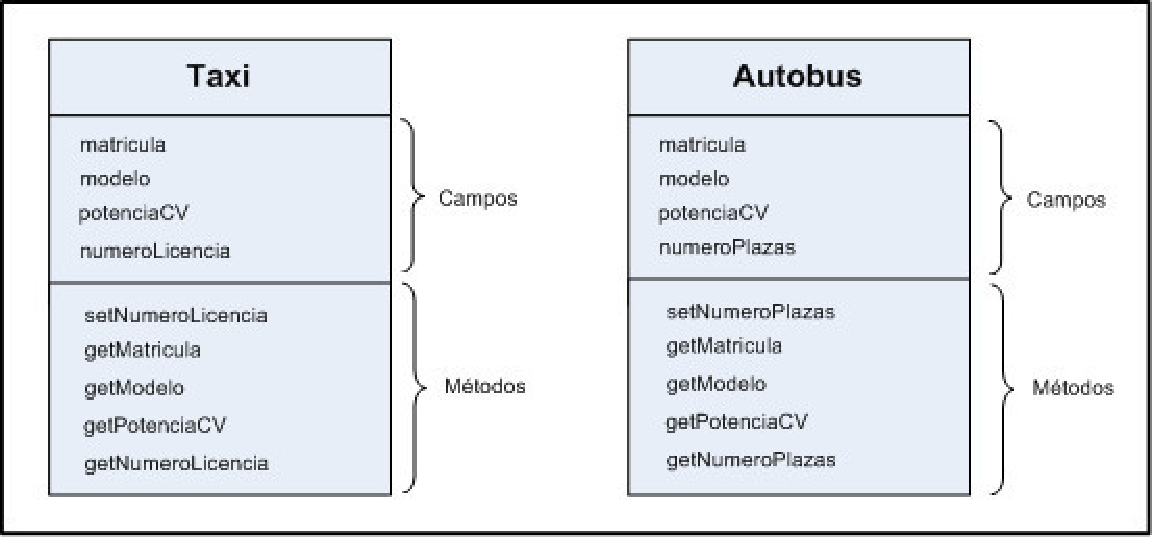
\includegraphics[width=10cm]{images/herencia_1.pdf}
			\end{center}
		\end{frame}

		\begin{frame}
			\frametitle{Conceptos}
			\framesubtitle{Herencia}
		
			\begin{center}
				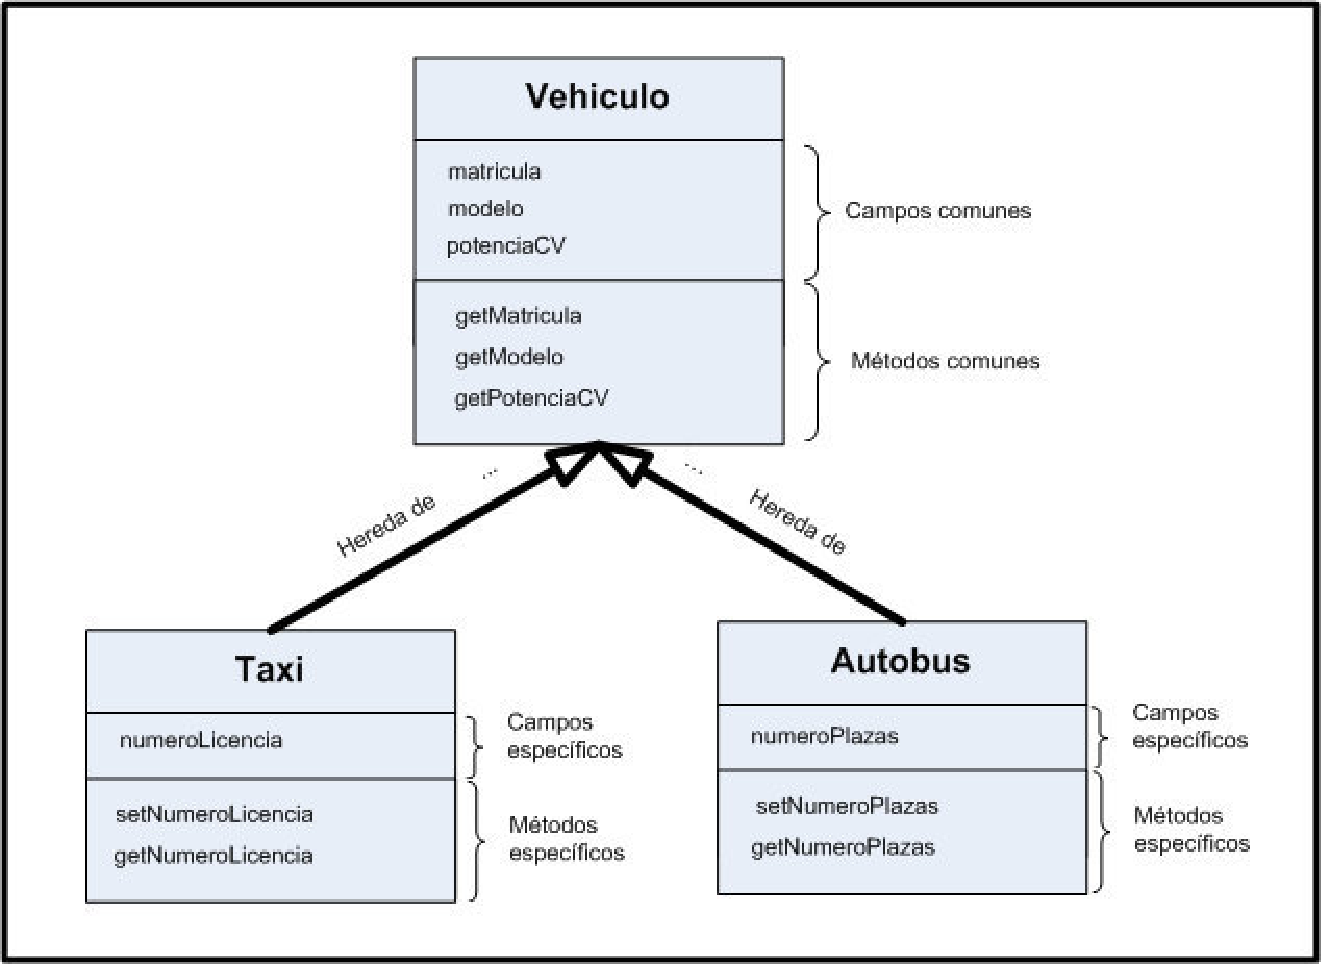
\includegraphics[width=8cm]{images/herencia_2.pdf}
			\end{center}
		\end{frame}

		\begin{frame}
			\frametitle{Conceptos}
			\framesubtitle{Herencia}

			\begin{block}{Introducci\'on}
				\begin{itemize}
  					\item Cuando una clase deriva de otra, hereda todos los atributos y m\'etodos (siempre y cuando sean definidos como \textbf{public} o \textbf{protected}).
					\item Estos m\'etodos y atributos, pueden ser redefinidos (\textbf{overridden}), en la clase derivada (sub-clase).
					\item Adem\'as, la clase derivada o sub-clase, puede agregar nuevos m\'etodos.
					\item En cierto modo puede confundir la idea de que la sub-clase \textbf{contenga} un objeto de la super-clase, pero la verdad es que la sub-case \textbf{ampl\'ia} la super-clase.
				\end{itemize}
			\end{block}
		\end{frame}

		\begin{frame}
			\frametitle{Conceptos}
			\framesubtitle{Herencia}

			\begin{block}{Introducci\'on}
				\begin{itemize}
  					\item JAVA permite m\'ultiples niveles de herencia, pero no permite que una clase derive de varias (\textbf{{\em no es posible la herencia m\'ultiple}}). Se pueden crear tantas clases derivadas de una misma clase como se quiera.
					\item Todas las clases de JAVA tienen una super-clase. Cuando no se indica expl\'icitamente una super-clase con la palabra  \textbf{extends}, la clase deriva de  \textbf{java.lang.Object},que es la clase ra\'iz de toda la jerarqu\'ia de clases de Java. Como consecuencia, todas las clases tienen m\'etodos que han heredado de \textbf{Object}.
				\end{itemize}
			\end{block}
		\end{frame}

		\begin{frame}
			\frametitle{Conceptos}
			\framesubtitle{Herencia}

			\begin{block}{Introducci\'on}
				\begin{itemize}
  					\item Una clase puede redefinir (volver a definir) cualquiera de los m\'etodos heredados de su super-clase que no sean \textbf{final}. El nuevo m\'etodo sustituye al heredado para todos los efectos en la clase que lo ha redefinido.
					\item Las m\'etodos de la super-clase que han sido redefinidos pueden ser todav\'ia accedidos por medio de la palabra \textbf{super} desde los m\'etodos de la clase derivada, aunque con este sistema s\'olo se puede subir un nivel en la jerarqu\'ia de clases.
				\end{itemize}
			\end{block}
		\end{frame}

		\subsection{Clases abstractas}

		\begin{frame}
			\frametitle{Conceptos}
			\framesubtitle{Clases abstractas}

			\begin{block}{Introducci\'on}
				\begin{itemize}
  					\item Los lenguajes de programaci\'on permiten expresar la soluci\'on de un problema de forma comprensible simult\'aneamente por la m\'aquina y el humano. 
					\item Constituyen un puente entre la abstracci\'on de la mente y una serie de instrucciones ejecutables.
					\item En consecuencia, la capacidad de abstracci\'on es una caracter\'istica deseable de los lenguajes de programaci\'on, pues cuanto mayor sea, mayor ser\'a su aproximaci\'on al lado humano.
				\end{itemize}
			\end{block}
		\end{frame}

		\begin{frame}
			\frametitle{Conceptos}
			\framesubtitle{Clases abstractas}

			\begin{block}{Una clase abstracta}
				\begin{itemize}
  					\item No permite instanciar o crear objetos de si misma.
					\item Su utilidad es permitir que otras clases deriven de ella, proporcionando un marco o modelo a seguir y m\'etodos de utilidad general.
					\item Las clases abstractas se declaran anteponiendo la palabra reservada \textbf{abstract}. Ejemplo:
					\begin{itemize}
  						\item \textbf{public} \textbf{abstract} \textbf{class} className \{ ...
					\end{itemize}
				\end{itemize}
			\end{block}
		\end{frame}
	
		\begin{frame}
			\frametitle{Conceptos}
			\framesubtitle{Clases abstractas}

			\begin{block}{Una clase abstracta}
				\begin{itemize}
  					\item Una clase abstracta puede tener m\'etodos declarados como \textbf{abstract}, en cuyo caso no se da la definici\'on del m\'etodo, m\'as si si declaraci\'on.
					\item Si una clase tiene al menos un m\'etodo de tipo \textbf{abstract}, la clase debe ser declarada como \textbf{abstract}.
					\item En toda sub-clase este m\'etodo deber\'a ser:
					\begin{itemize}
  						\item Redefinido (volver a declararlo como \textbf{abstract}, al igual que la sub-clase).
						\item Implementarlo.
					\end{itemize}
					\item Una clase abstracta puede tener m\'etodos declarados como no abstracto. En este caso, la sub-clase hereda el m\'etodo completamente para ser utilizado.
				\end{itemize}
			\end{block}
		\end{frame}

		\subsection{Interfaz}

		\begin{frame}
			\frametitle{Conceptos}
			\framesubtitle{Interfaz}

			\begin{block}{Concepto de interfaz}
				\begin{itemize}
  					\item Una interface es un conjunto de declaraciones de m\'etodos (sin definici\'on). 
					\item Tambi\'en puede definir constantes, que son impl\'icitamente \textbf{public}, \textbf{static} y \textbf{final}, y deben siempre inicializarse en la declaraci\'on.
					\item Estos m\'etodos definen un tipo de {\em comportamiento}.
					\item Todas las clases que implementan una determinada interface est\'an obligadas a proporcionar una definici\'on de los m\'etodos de la interface, y en ese sentido adquieren una conducta o modo de funcionamiento.
				\end{itemize}
			\end{block}
		\end{frame}

		\begin{frame}
			\frametitle{Conceptos}
			\framesubtitle{Interfaz}

			\begin{block}{Concepto de interfaz}
				\begin{itemize}
  					\item Una clase puede implementar una o varias interfaces. 
					\item Para indicar que una clase implementa una o m\'as interfaces se ponen los nombres de las interfaces, separados por comas, detr\'as de la palabra reservada \textbf{implements}, que a su vez va siempre a la derecha del nombre de la clase o del nombre de la super-clase en el caso de herencia. 
					\item Por ejemplo,
					\begin{itemize}
  						\item public class className \textbf{implements} interfaceName1, interfaceName2, ... \{ ...
					\end{itemize}	
				\end{itemize}
			\end{block}
		\end{frame}

		\begin{frame}
			\frametitle{Conceptos}
			\framesubtitle{Interfaz}

			\begin{block}{Interfaz v/s clase abstract}
				\begin{itemize}
  					\item Ambas pueden contener varias declaraciones de m\'etodos (la clase abstract puede adem\'as definir otros). 
					\item Una clase no puede heredar de dos clases abstract, pero s\'i puede heredar de una clase abstract e implementar una interface, o bien implementar dos o m\'as interfaces.
					\item Las interfaces permiten mucha m\'as flexibilidad para conseguir que dos clases tengan el mismo comportamiento, inpendientemente de su situaci\'on en la jerarqu\'ia de clases de JAVA.
					\item Las interfaces permiten ''publicar'' el comportamiento de una clase desvelando un m\'inimo de informaci\'on.
				\end{itemize}
			\end{block}
		\end{frame}    
    
		\begin{frame}
			\frametitle{Conceptos}
			\framesubtitle{Ejercicio}

			\begin{exampleblock}{Ejercicio}
			{\scriptsize
				Se plantea desarrollar un programa Java que permita la gesti\'on de una empresa de alimentos que trabaja con tres tipos de productos: productos frescos, productos refrigerados y productos congelados. Todos los productos llevan esta informaci\'on com\'un: fecha de caducidad y n\'umero de lote. A su vez, cada tipo de producto lleva alguna informaci\'on espec\'ifica. Los productos frescos deben llevar la fecha de envasado y el pa\'is de origen. Los productos refrigerados deben llevar el c\'odigo del organismo de supervisi\'on alimentaria. Los productos congelados deben llevar la temperatura de congelaci\'on recomendada. Crear el c\'odigo de las clases Java implementando una relaci\'on de herencia desde la superclase \textbf{Producto} hasta las subclases \textbf{ProductoFresco}, \textbf{ProductoRefrigerado} y \textbf{ProductoCongelado}. Cada clase debe disponer de constructor, permitir establecer y recuperar el valor de sus atributos y tener un m\'etodo que permita mostrar la informaci\'on del objeto \emph{(toString)}. Crear una clase principal con el m\'etodo \emph{main} donde se cree un objeto de cada tipo y se ingresen y muestren los datos de cada uno de los objetos creados.}
			\end{exampleblock}
		\end{frame}       

        \begin{frame}
			\frametitle{Conceptos}
			\framesubtitle{Ejercicio}

			\begin{exampleblock}{Ejercicio}
				Se requiere desarrollar un sistema de apoyo a la docencia de geometr\'ia matem\'aticas. Para ello, se debe definir una categorizaci\'n de figuras geom\'etricas, por ahora s\'olo Cuadrados, Tri\'angulos y Circunferencias. Para cada uno de ellos se debe calcular el per\'imetro y el \'area. Es relevante para el sistema mostrar la informaci\'on de la figura geom\'etrica a trav\'es de alg\'un m\'etodo. Desarrolle este sistema en JAVA utilizando el conceto de herencia, implementado una interfaz para las figuras geom\'etricas.
			\end{exampleblock}
		\end{frame}           
    
	\section{Tipos de datos abstractos}

		\subsection{Definici\'on}

		\begin{frame}
			\frametitle{Tipos de datos abstractos}
			\framesubtitle{Definici\'on}

			\begin{block}{Definici\'on}
				Es un modelo compuesto por una colecci\'on de operaciones definidas sobre un conjunto de datos para el modelo.
			\end{block}
			\begin{block}{Ejemplos de usos de TDA}
				\textbf{Conjuntos}: Implementaci\'on de conjuntos con sus operaciones b\'asicas (uni\'on, intersecci\'on y diferencia), operaciones de inserci\'on, borrado, b\'usqueda...\\
				\textbf{\'Arboles Binarios de B\'usqueda}: Implementaci\'on de \'arboles de elementos, utilizados para la representaci\'on interna de datos complejos. Aunque siempre se los toma como un TDA separado son parte de la familia de los grafos. \\
				\textbf{Pilas y Colas}: Implementaci\'on de los algoritmos FIFO y LIFO. \\
				\textbf{Grafos}: V\'ertices unidos mediante arcos o aristas.
			\end{block}
		\end{frame}

		\subsection{Bean}

		\begin{frame}
			\frametitle{Tipos de datos abstractos}
			\framesubtitle{Beans}

			\begin{block}{Definici\'on}
				Un Bean es un componente software que tiene la particularidad de ser reutilizable y as\'i evitar la tediosa tarea de reescribir los distintos componentes uno a uno.
			\end{block}
			\begin{block}{Criterios que debe cumplir un Bean}
				\begin{itemize}
  					\item Un Bean debe cumplir los siguientes criterios:
					\begin{itemize}
						\item Tener todos sus atributos privados (private).
						\item Tener m\'etodos set() y get() p\'ublicos de los atributos privados.
						\item Tener un constructor p\'ublico por defecto (opcional).
					\end{itemize}
				\end{itemize}
			\end{block}
		\end{frame}

		\begin{frame}
			\frametitle{Tipos de datos abstractos}
			\framesubtitle{Beans}

			\begin{block}{Ejemplo}
				Considere los datos de una persona como atributos de una clase. Cree una clase Bean denominada \textbf{Persona}, que implemente los m\'etodos get() y set() y el constructor m\'as apropiado.
			\end{block}
		\end{frame}

		\subsection{Listas}

		\begin{frame}
			\frametitle{Tipos de datos abstractos}
			\framesubtitle{Listas}

			\begin{block}{Definici\'on Nodos}
				\begin{itemize}
					\item Toda lista est\'a compuesta por nodos:
					\begin{itemize}
						\item Se denomina nodo, elemento o \'item, a la unidad de informaci\'an m\'as elemental o indivisible dentro de una lista.
					\end{itemize}
					\item Una lista lineal es un conjunto de {\em \textbf{n}} nodos con n $\geq$ 0, cuyas propiedades estructurales esenciales incluyen s\'olo las posiciones lineales relativas de los nodos.
				\end{itemize}
			\end{block}
		\end{frame}

		\begin{frame}
			\frametitle{Tipos de datos abstractos}
			\framesubtitle{Listas}

			\begin{block}{Algunas operaciones sobre las listas}
				\begin{itemize}
					\item Tener acceso a un nodo.
					\item Insertar y eliminar un nodo en la lista.
					\item Combinar dos o m\'as listas en una.
					\item Dividir una lista en dos o m\'as listas.
					\item Determinar la cantidad de nodos de la lista.
					\item Ordenar la lista de acuerdo a un criterio.
					\item Buscar un elemento bajo una condici\'on.
					\item Etc.
				\end{itemize}
			\end{block}
		\end{frame}

		\begin{frame}
			\frametitle{Tipos de datos abstractos}
			\framesubtitle{Listas}

			\begin{block}{Consideraciones sobre las listas}
				\begin{itemize}
					\item $n = 0$ denota a la lista vac\'ia, o sea, una lista que no tiene elementos.
					\item Si $n > 0$, $l_{0}$ es el primer nodo.
					\item Si $1 > k > n$, $l_{k}$ es precedido por el nodo $l_{k-1}$ y seguido por el nodo $l_{k+1}$.
					\item Si $n > 0$, $I_{n-1}$ es el \'ultimo nodo.
				\end{itemize}
			\end{block}
		\end{frame}
		
		\begin{frame}
			\frametitle{Tipos de datos abstractos}
			\framesubtitle{Listas}

			\begin{block}{Consideraciones sobre las listas}
				\begin{itemize}
					\item En una lista se asigna memoria para el almacenar los elementos, conforme se va necesitando, es decir a medida que se a\~naden o insertan los elementos, y se conectan los elementos de la lista con punteros. 
					\item La memoria es liberada cuando ya no se necesita m\'as un elemento en la lista. 
					\item Esquem\'aticamente una lista enlazada se representa por una secuencia de nodos conectados por enlaces.
				\end{itemize}
			\end{block}
		\end{frame}

		\begin{frame}
			\frametitle{Tipos de datos abstractos}
			\framesubtitle{Listas}

			\begin{block}{Esquema g\'afico de las listas}
				\begin{center}
					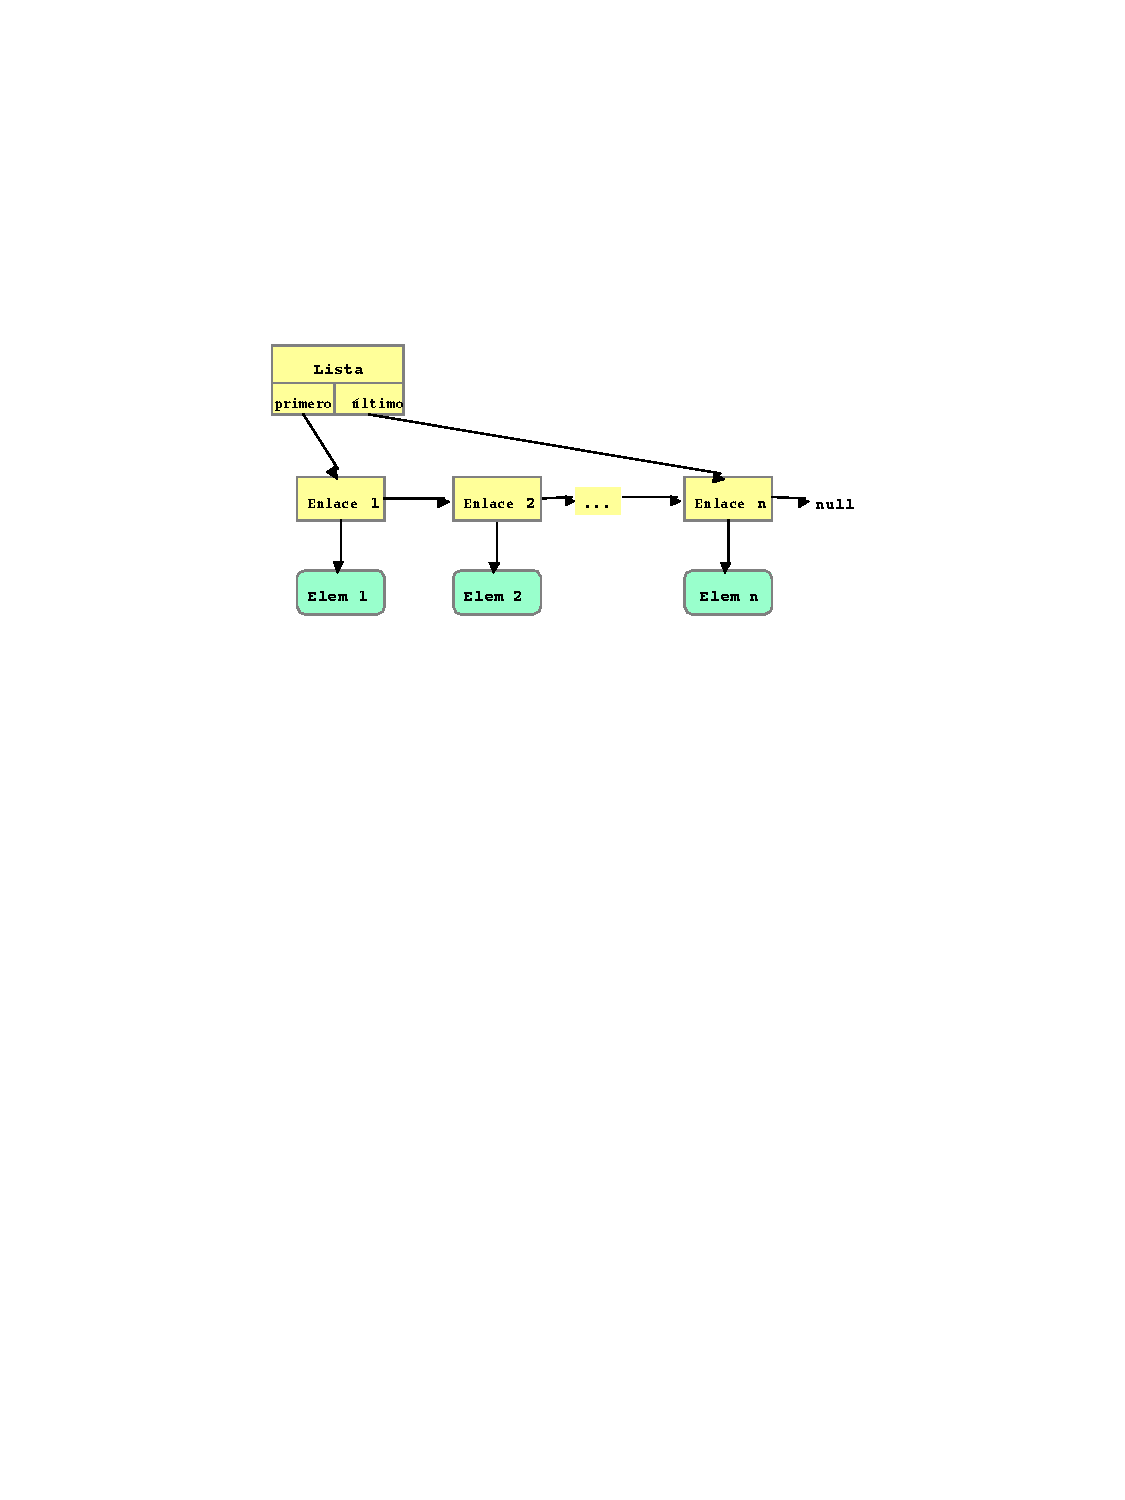
\includegraphics[width=10cm]{images/esquema.pdf}
				\end{center}
			\end{block}
		\end{frame}

		\begin{frame}
			\frametitle{Tipos de datos abstractos}
			\framesubtitle{Listas}

			\begin{block}{Interface List}
				\textbf{public interface} List \{ \\
				\ \ \ \ \textbf{public abstract boolean} isEmpty(); \\ 
				\ \ \ \ \textbf{public abstract void} add(\textbf{Object} o); \\
				\ \ \ \ \textbf{public abstract boolean} contains(\textbf{Object} o); \\ 
				\ \ \ \ \textbf{public abstract boolean} remove(\textbf{Object} o); \\
				\ \ \ \ \textbf{public abstract void} clear(); \\
				\ \ \ \ \textbf{public abstract int} size(); \\
				\ \ \ \ \textbf{public abstract List} subList(\textbf{int} firstIndex, \textbf{int} lastIndex); \\
				\ \ \ \ ... \\
				\}
			\end{block}
		\end{frame}	

		\begin{frame}
			\frametitle{Tipos de datos abstractos}
			\framesubtitle{Listas}

			\begin{block}{Implementaci\'on de la interface List}
				\textbf{Vector v/s ArrayList } \\
				\textbf{Sincronizaci\'on}: La clase \textbf{Vector} es sincronizada (synchronized) y, por tanto, su contenido est\'a protegido de otros hilos, es decir, es thread-safe. Por al contrario, los \textbf{ArrayList} no son sincronizados y por tanto no son thread-safe. \\
				Se debe tener en cuanta esto porque los \textbf{Vectores} tienen un costo en tiempo de ejecuci\'on que no tienen los \textbf{ArrayList}. Si no se necesita thead-safe, se utiliza \textbf{ArrayList}.
			\end{block}
		\end{frame}

		\begin{frame}
			\frametitle{Tipos de datos abstractos}
			\framesubtitle{Listas}

			\begin{block}{Implementaci\'on de la interface List}
				\begin{itemize}
					\item Implementaci\'on con \textbf{Vector} 
					\begin{itemize}
						\item \textbf{List} lista = \textbf{new Vector ()}; 
						\item \textbf{List $<$Class$>$} lista = \textbf{new Vector $<$Class$>$ ()}; 
					\end{itemize}
					\item Implementaci\'on con \textbf{ArrayList} 
					\begin{itemize}
						\item \textbf{List} lista = \textbf{new ArrayList ()}; 
						\item \textbf{List $<$Class$>$} lista = \textbf{new ArrayList $<$Class$>$ ()}; 
					\end{itemize}
					\item Como nueva norma o est\'andar se adopt\'o especificar el tipo de objetos que se almacenar\'a en las listas a diferencia de las listas gen\'ericas que antiguamente se creaban.
				\end{itemize}
			\end{block}
		\end{frame}    
    
    \section{Fuente de datos}

		\subsection{Definici\'on}

		\begin{frame}
			\frametitle{Fuente de datos}
			\framesubtitle{Archivos - Definici\'on}

			\begin{block}{Definici\'on}
				\begin{itemize}
					\item Un archivo es un conjunto de bits almacenado en un dispositivo.
					\item Un archivo es identificado por un nombre y la descripci\'on del directorio que lo contiene.
					\item Los archivos proporcionan una manera de organizar los recursos usados para almacenar permanentemente datos en un sistema inform\'atico.
				\end{itemize}
			\end{block}
		\end{frame}

		\subsection{Lectura de archivos en JAVA}

		\begin{frame}
			\frametitle{Fuente de datos}
			\framesubtitle{Lectura de archivos en JAVA}

			\begin{block}{Consideraciones}
				\begin{itemize}
					\item El proceso de lectura de un archivo en JAVA, es similar a la lectura desde el dispositivo est\'andar (teclado). 
					\item Creamos un objeto entrada de la clase \textbf{FileReader} en vez de \textbf{InputStreamReader}. 
					\item El final del archivo viene dado cuando la funci\'on \textbf{readLine} retorna \textbf{{\em null}}. 
					\item El resto del c\'odigo es similar.
				\end{itemize}
			\end{block}
		\end{frame}

		\begin{frame}
			\frametitle{Fuente de datos}
			\framesubtitle{Ejemplo}

			\begin{block}{Ejemplo}
			{\scriptsize
				\textbf{public void} readFile() \{ \\
				\ \ \ \ \textbf{File} archivo = \textbf{null}; \\ 
			         \ \ \ \ \textbf{FileReader} fileReader = \textbf{null};\\
				\ \ \ \ \textbf{try} \{ \\
                       		\ \ \ \ \ \ \ \ archivo = new \textbf{File} (''archivo.txt''); \\
				\ \ \ \ \ \ \ \ String linea; \\
				\ \ \ \ \ \ \ \ fileReader = new \textbf{FileReader} (archivo); \\
				\ \ \ \ \ \ \ \ \textbf{BufferedReader} br = new \textbf{BufferedReader} (fileReader); \\
				\ \ \ \ \ \ \ \ \textbf{while}((linea = br.readLine()) != \textbf{null}) \{ \\
				\ \ \ \ \ \ \ \ \ \ \ \ System.out.println(linea); \\
				\ \ \ \ \ \ \ \ \ \} \\
				\ \ \ \ \} \\
			}
			\end{block}
		\end{frame}

		\begin{frame}
			\frametitle{Fuente de datos}
			\framesubtitle{Ejemplo - Continuaci\'on}

			\begin{block}{Ejemplo  - Continuaci\'on}
			{\scriptsize
				\ \ \ \ \textbf{catch} (IOException e) \{ \\
                                     \ \ \ \ \ \ \ \ System.out.println(e); \\
                                     \ \ \ \ \} \\
                                     \ \ \ \ \textbf{finally} \{ \\
                                     \ \ \ \ \ \ \ \ \textbf{try} \{ \\
                                     \ \ \ \ \ \ \ \ \ \ \ \ \textbf{if} (fileReader !=  \textbf{null}) \{ \\
                                     \ \ \ \ \ \ \ \ \ \ \ \ \ \ \ \ fileReader.close(); \\
                                     \ \ \ \ \ \ \ \ \ \ \ \ \} \\
                                     \ \ \ \ \ \ \ \ \} \\
                                     \ \ \ \ \ \ \ \ \textbf{catch} (IOException e) \{ \\
                                     \ \ \ \ \ \ \ \ \ \ \ \ System.out.println(e); \\
                                     \ \ \ \ \ \ \ \ \}\\
                                     \ \ \ \ \} \\
                                     \}
			}
			\end{block}
		\end{frame}

		\subsection{Escritura de archivos en JAVA}

		\begin{frame}
			\frametitle{Fuente de datos}
			\framesubtitle{Escritura de archivos en JAVA}

			\begin{block}{Consideraciones}
				\begin{itemize}
					\item Creamos un objeto de entrada de la clase \textbf{FileWriter}. 
					\item Si queremos a\~nadir al final de un fichero ya existente, simplemente debemos agregar un flag a \textbf{true} como segundo par\'ametro del constructor de \textbf{FileWriter}.
				\end{itemize}
			\end{block}
		\end{frame}

		\begin{frame}
			\frametitle{Fuente de datos}
			\framesubtitle{Ejemplo}

			\begin{block}{Ejemplo}
			{\scriptsize
				\textbf{public void} writeFile() \{ \\
				\ \ \ \ \textbf{FileWriter} archivo = \textbf{null}; \\ 
			         \ \ \ \ \textbf{PrintWriter} printWriter = \textbf{null};\\
				\ \ \ \ \textbf{try} \{ \\
                       		\ \ \ \ \ \ \ \ archivo = new \textbf{FileWriter} (''archivo.txt''); \\
				\ \ \ \ \ \ \ \ printWriter = new \textbf{PrintWriter} (archivo); \\
				\ \ \ \ \ \ \ \ \textbf{for}(\textbf{int} count = 0; count $<$ 10; count++) \{ \\
				\ \ \ \ \ \ \ \ \ \ \ \ printWriter.println ('Linea: '' + count); \\
				\ \ \ \ \ \ \ \ \ \} \\
				\ \ \ \ \} \\
			}
			\end{block}
		\end{frame}

		\begin{frame}
			\frametitle{Fuente de datos}
			\framesubtitle{Ejemplo - Continuaci\'on}

			\begin{block}{Ejemplo  - Continuaci\'on}
			{\scriptsize
				\ \ \ \ \textbf{catch} (IOException e) \{ \\
                                     \ \ \ \ \ \ \ \ System.out.println(e); \\
                                     \ \ \ \ \} \\
                                     \ \ \ \ \textbf{finally} \{ \\
                                     \ \ \ \ \ \ \ \ \textbf{try} \{ \\
                                     \ \ \ \ \ \ \ \ \ \ \ \ printWriter.close(); \\
                                     \ \ \ \ \ \ \ \ \} \\
                                     \ \ \ \ \ \ \ \ \textbf{catch} (IOException e) \{ \\
                                     \ \ \ \ \ \ \ \ \ \ \ \ System.out.println(e); \\
                                     \ \ \ \ \ \ \ \ \}\\
                                     \ \ \ \ \} \\
                                     \}
			}
			\end{block}
		\end{frame}
    
\end{document}

\usetheme{default}
\usetheme{JuanLesPins}
\usetheme{Goettingen}
\usetheme{Szeged}
\usetheme{Warsaw}

\usecolortheme{crane}

\usefonttheme{serif}
\usefonttheme{structuresmallcapsserif}